% Source: StudentGovernmentRepo/Common_Sense_Carolina_Lobbying_org/figures/org_phase5.tex
\documentclass[border=15pt]{standalone}
\usepackage{tikz}
\usepackage{xcolor}
\usetikzlibrary{positioning, arrows.meta, calc, fit, backgrounds}
\definecolor{garnet}{HTML}{73000A}
\definecolor{lightgarnet}{HTML}{F5EAEB}
\definecolor{sandstorm}{HTML}{FFF2E3}
\definecolor{rose}{HTML}{CC2E40}
\definecolor{atlantic}{HTML}{466A9F}
\definecolor{congaree}{HTML}{1F414D}
\definecolor{horseshoe}{HTML}{65780B}
\definecolor{honeycomb}{HTML}{A49137}
\definecolor{grass}{HTML}{CED318}
\definecolor{warmgrey}{HTML}{676156}
\definecolor{tenblack}{HTML}{ECECEC}

\begin{document}
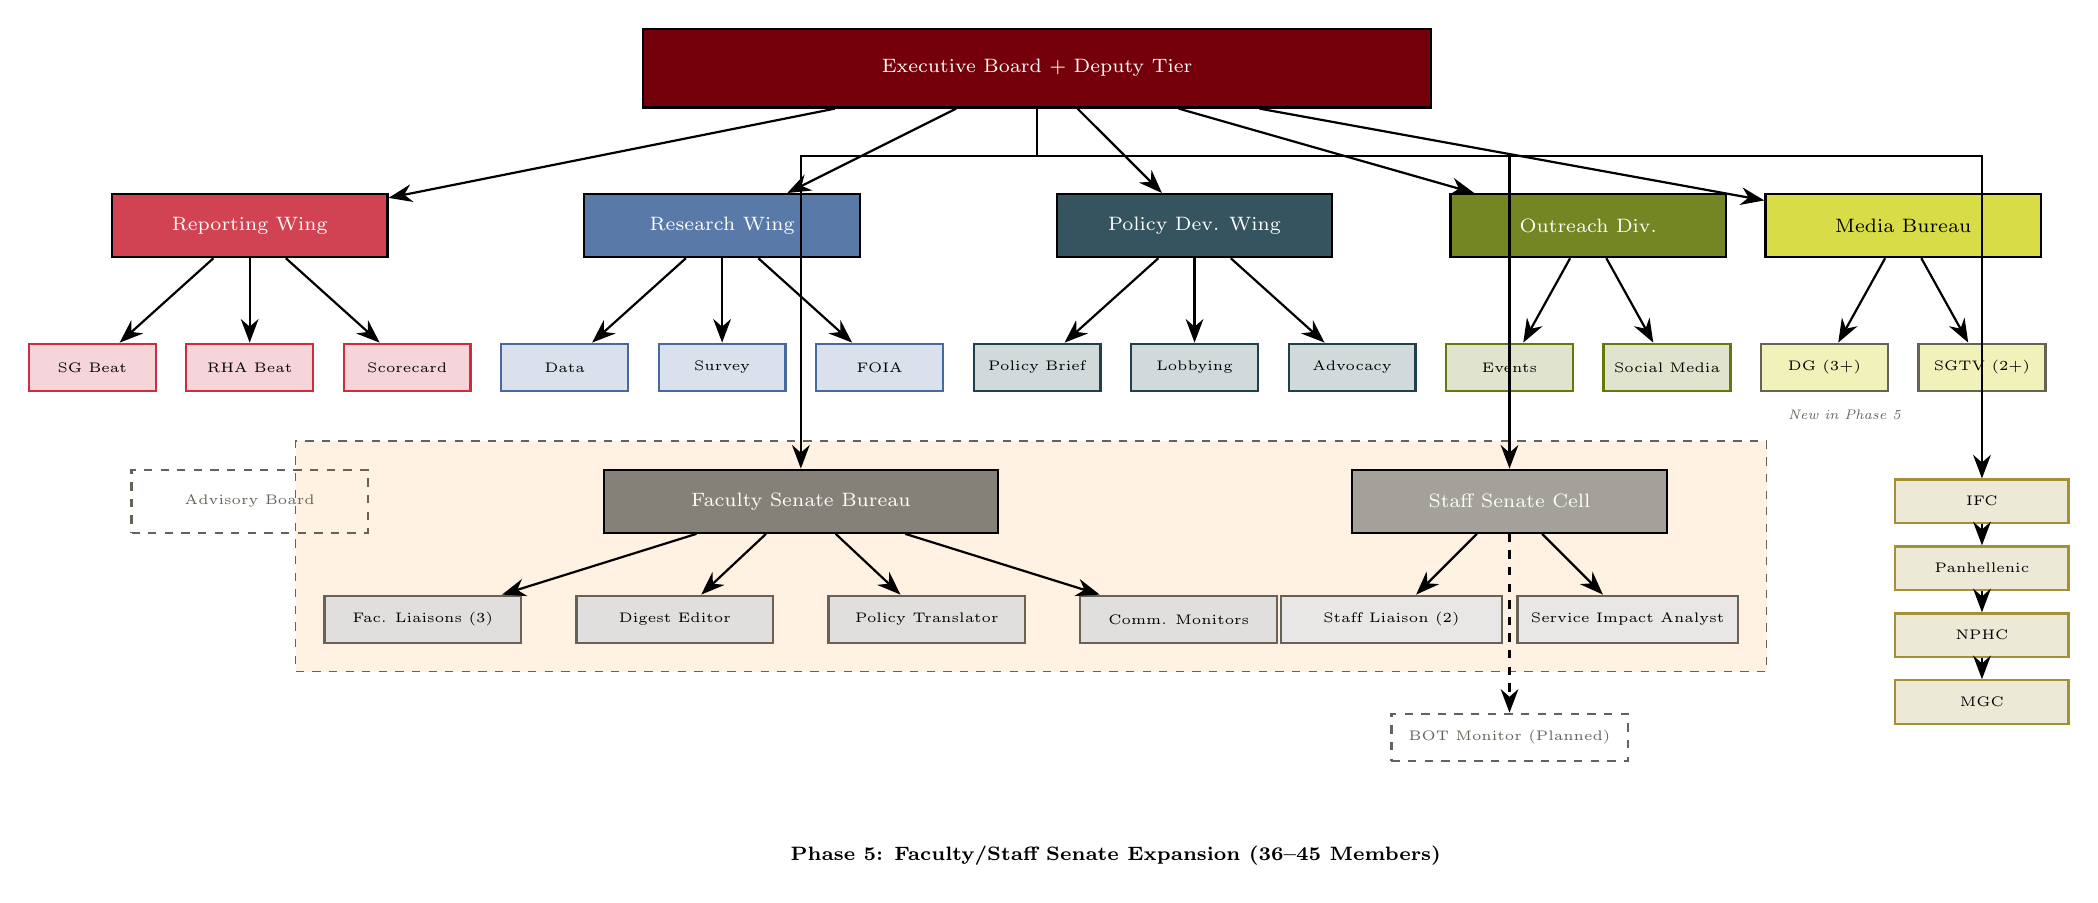
\begin{tikzpicture}[
  >=Stealth,
  thick,
  every node/.style={rectangle, draw, align=center, sharp corners},
  arr/.style={-{Stealth[length=3mm]}, thick},
  %% Leaf node: text width=1.4cm forces wrapping, inner sep=3pt.
  %% Rendered width = 1.4cm + 2*0.1cm = ~1.6cm.
  %% Center-to-center spacing = 2.0cm => 0.4cm gap between adjacent boxes.
  leaf/.style={minimum height=0.6cm, inner sep=3pt, font=\tiny, text width=1.4cm}
]

%% ─── Row 0: Executive Board (y=0) ──────────────────────────────────────────
\node[fill=garnet, text=white, minimum width=10cm, minimum height=1cm,
      font=\scriptsize] (exec) at (0,0)
  {Executive Board + Deputy Tier};

%% ─── Row 1: Wings (y=-2) ────────────────────────────────────────────────────
%% Centered over their respective sub-item groups
\node[fill=rose!90, text=white, minimum width=3.5cm, minimum height=0.8cm,
      font=\scriptsize] (rep) at (-10,-2) {Reporting Wing};

\node[fill=atlantic!90, text=white, minimum width=3.5cm, minimum height=0.8cm,
      font=\scriptsize] (res) at (-4,-2) {Research Wing};

\node[fill=congaree!90, text=white, minimum width=3.5cm, minimum height=0.8cm,
      font=\scriptsize] (pol) at (2,-2) {Policy Dev. Wing};

\node[fill=horseshoe!90, text=white, minimum width=3.5cm, minimum height=0.8cm,
      font=\scriptsize] (out) at (7,-2) {Outreach Div.};

\node[fill=grass!80, text=black, minimum width=3.5cm, minimum height=0.8cm,
      font=\scriptsize] (med) at (11,-2) {Media Bureau};

%% Row 0 to Row 1 arrows
\draw[arr] (exec) -- (rep);
\draw[arr] (exec) -- (res);
\draw[arr] (exec) -- (pol);
\draw[arr] (exec) -- (out);
\draw[arr] (exec) -- (med);

%% ─── Row 2: Sub-items (y=-3.8) ──────────────────────────────────────────────
%% 13 nodes in a single row, uniform 2.0cm center-to-center spacing.
%% Positions: -12, -10, -8, -6, -4, -2, 0, 2, 4, 6, 8, 10, 12

%% Under Reporting Wing (center=-10)
\node[leaf, fill=rose!20, draw=rose]
  (rep1) at (-12,-3.8) {SG Beat};
\node[leaf, fill=rose!20, draw=rose]
  (rep2) at (-10,-3.8) {RHA Beat};
\node[leaf, fill=rose!20, draw=rose]
  (rep3) at (-8,-3.8) {Scorecard};

\draw[arr] (rep) -- (rep1);
\draw[arr] (rep) -- (rep2);
\draw[arr] (rep) -- (rep3);

%% Under Research Wing (center=-4)
\node[leaf, fill=atlantic!20, draw=atlantic]
  (res1) at (-6,-3.8) {Data};
\node[leaf, fill=atlantic!20, draw=atlantic]
  (res2) at (-4,-3.8) {Survey};
\node[leaf, fill=atlantic!20, draw=atlantic]
  (res3) at (-2,-3.8) {FOIA};

\draw[arr] (res) -- (res1);
\draw[arr] (res) -- (res2);
\draw[arr] (res) -- (res3);

%% Under Policy Dev. Wing (center=2)
\node[leaf, fill=congaree!20, draw=congaree]
  (pol1) at (0,-3.8) {Policy Brief};
\node[leaf, fill=congaree!20, draw=congaree]
  (pol2) at (2,-3.8) {Lobbying};
\node[leaf, fill=congaree!20, draw=congaree]
  (pol3) at (4,-3.8) {Advocacy};

\draw[arr] (pol) -- (pol1);
\draw[arr] (pol) -- (pol2);
\draw[arr] (pol) -- (pol3);

%% Under Outreach Div. (center=7)
\node[leaf, fill=horseshoe!20, draw=horseshoe]
  (out1) at (6,-3.8) {Events};
\node[leaf, fill=horseshoe!20, draw=horseshoe]
  (out2) at (8,-3.8) {Social Media};

\draw[arr] (out) -- (out1);
\draw[arr] (out) -- (out2);

%% Under Media Bureau (center=11)
\node[leaf, fill=grass!30, draw=warmgrey]
  (med1) at (10,-3.8) {DG (3+)};
\node[leaf, fill=grass!30, draw=warmgrey]
  (med2) at (12,-3.8) {SGTV (2+)};

\draw[arr] (med) -- (med1);
\draw[arr] (med) -- (med2);

%% ─── Advisory Board (y=-5.5, x=-10) ─────────────────────────────────────────
\node[draw=warmgrey, dashed, fill=none, minimum width=3cm, minimum height=0.8cm,
      font=\tiny, text=warmgrey] (adv) at (-10,-5.5) {Advisory Board};

%% ─── Row 3: Faculty Senate Bureau header (y=-5.5, x=-3) ────────────────────
\node[fill=warmgrey!80, text=white, minimum width=5cm, minimum height=0.8cm,
      font=\scriptsize] (fsbhdr) at (-3,-5.5) {Faculty Senate Bureau};

\draw[arr] (exec.south) -- ++(0,-0.6) -| (fsbhdr.north);

%% Faculty Bureau sub-items (y=-7)
%% 4 nodes, min width=2.5cm + inner sep ~5pt => ~2.85cm rendered.
%% Spacing = 3.2cm center-to-center.
\node[fill=warmgrey!20, draw=warmgrey, minimum width=2.5cm, minimum height=0.6cm,
      font=\tiny] (fs1) at (-7.8,-7) {Fac. Liaisons (3)};
\node[fill=warmgrey!20, draw=warmgrey, minimum width=2.5cm, minimum height=0.6cm,
      font=\tiny] (fs2) at (-4.6,-7) {Digest Editor};
\node[fill=warmgrey!20, draw=warmgrey, minimum width=2.5cm, minimum height=0.6cm,
      font=\tiny] (fs3) at (-1.4,-7) {Policy Translator};
\node[fill=warmgrey!20, draw=warmgrey, minimum width=2.5cm, minimum height=0.6cm,
      font=\tiny] (fs4) at (1.8,-7) {Comm. Monitors};

\draw[arr] (fsbhdr) -- (fs1);
\draw[arr] (fsbhdr) -- (fs2);
\draw[arr] (fsbhdr) -- (fs3);
\draw[arr] (fsbhdr) -- (fs4);

%% ─── Row 3: Staff Senate Cell header (y=-5.5, x=6) ─────────────────────────
\node[fill=warmgrey!60, text=white, minimum width=4cm, minimum height=0.8cm,
      font=\scriptsize] (sschdr) at (6,-5.5) {Staff Senate Cell};

\draw[arr] (exec.south) -- ++(0,-0.6) -| (sschdr.north);

%% Staff Cell sub-items (y=-7)
\node[fill=warmgrey!15, draw=warmgrey, minimum width=2.8cm, minimum height=0.6cm,
      font=\tiny] (ss1) at (4.5,-7) {Staff Liaison (2)};
\node[fill=warmgrey!15, draw=warmgrey, minimum width=2.8cm, minimum height=0.6cm,
      font=\tiny] (ss2) at (7.5,-7) {Service Impact Analyst};

\draw[arr] (sschdr) -- (ss1);
\draw[arr] (sschdr) -- (ss2);

%% ─── Row 4: BOT Monitor (y=-8.5, x=6) ──────────────────────────────────────
\node[draw=warmgrey, dashed, fill=none, minimum width=3cm, minimum height=0.6cm,
      font=\tiny, text=warmgrey] (bot) at (6,-8.5) {BOT Monitor (Planned)};

\draw[arr, dashed] (sschdr.south) -- (bot.north);

%% ─── Greek Liaisons column (x=12, y=-5.5 to -8) ────────────────────────────
\node[fill=honeycomb!20, draw=honeycomb, minimum width=2.2cm, minimum height=0.55cm,
      font=\tiny] (ifc)  at (12,-5.5)  {IFC};
\node[fill=honeycomb!20, draw=honeycomb, minimum width=2.2cm, minimum height=0.55cm,
      font=\tiny] (pan)  at (12,-6.35) {Panhellenic};
\node[fill=honeycomb!20, draw=honeycomb, minimum width=2.2cm, minimum height=0.55cm,
      font=\tiny] (nphc) at (12,-7.2)  {NPHC};
\node[fill=honeycomb!20, draw=honeycomb, minimum width=2.2cm, minimum height=0.55cm,
      font=\tiny] (mgc)  at (12,-8.05) {MGC};

\draw[arr] (exec.south) -- ++(0,-0.6) -| (ifc.north);
\draw[arr] (ifc)  -- (pan);
\draw[arr] (pan)  -- (nphc);
\draw[arr] (nphc) -- (mgc);

%% ─── Background highlight: New in Phase 5 ───────────────────────────────────
\begin{pgfonlayer}{background}
  \node[fill=sandstorm, draw=warmgrey, dashed, sharp corners,
        inner sep=10pt,
        fit=(fsbhdr)(sschdr)(fs1)(fs2)(fs3)(fs4)(ss1)(ss2)]
        (newbox) {};
\end{pgfonlayer}

\node[draw=none, fill=none, font=\tiny\itshape, text=warmgrey]
  at ([xshift=4pt, yshift=4pt] newbox.north east) [above right] {New in Phase 5};

%% ─── Title (y=-10) ──────────────────────────────────────────────────────────
\node[draw=none, fill=none, font=\scriptsize\bfseries] at (1,-10)
  {Phase 5: Faculty/Staff Senate Expansion (36--45 Members)};

\end{tikzpicture}
\end{document}
